\section{Data}
\label{sec:data}

We explore the behavior of the metrics on mock classifications with well-understood weaknesses as well as realistic mock classifications from past challenges.
Throughout the paper, ``data'' always refers to classification results, not lightcurves; no lightcurves were simulated, viewed, or classified in the preparation of this paper.
Data is in the form of catalogs of posterior probability vectors $p(m \mid d)$ over $M$ classes with labels $m$ conditioned on the observed lightcurve $d$, with each probability vector normalized to sum to unity.
We describe below the way in which mock data is synthesized.

First, we propose that the class populations are logarithmically distributed such that they span many orders of magnitude, as is anticipated for the real \lsst\ dataset.
%We then take $M$ draws $u_{m} \sim \mathcal{U}(0, 1)$ from the standard continuous uniform distribution and establish a discrete probability distribution $p(m) = b^{u_{m}}\ Z^{-1}$ where $Z = \sum_{m} b^{u_{m}}$, i.e. such that $\sum_{m=1}^{M} p(m) = 1$.
We then take $M$ draws $u_{m} \sim \mathcal{U}(0, 1)$ from the standard continuous uniform distribution. These coefficients $u_m$ define the discrete probability distribution for each class $m$ in $M:$ \begin{equation}p(m) = \frac{b^{u_{m}}}{\sum_{m} b^{u_{m}}},\end{equation} such that $\sum_{m=1}^{M} p(m) = 1$.
% was the b in 10^b really related to the b above? This was not clear.
We draw $N = 10^{b}$ instances $\{m'_{n}\}$ of a true class $m'$ for each lightcurve $n$ in the catalog from $p(m')$.
We used a distribution of $M=13$ true classes and chose $b=6$ used in our tests is shown in Figure~\ref{fig:classdist}, with the class labels ordered by their size. \textbf{[RH removed excess variables/symbols that made things more wordy than they need to be]}
Though the class labels for \plasticc\ will presumably be randomized, we use this ordering to ease visual inspection of our results.

\begin{figure}
	\begin{center}
    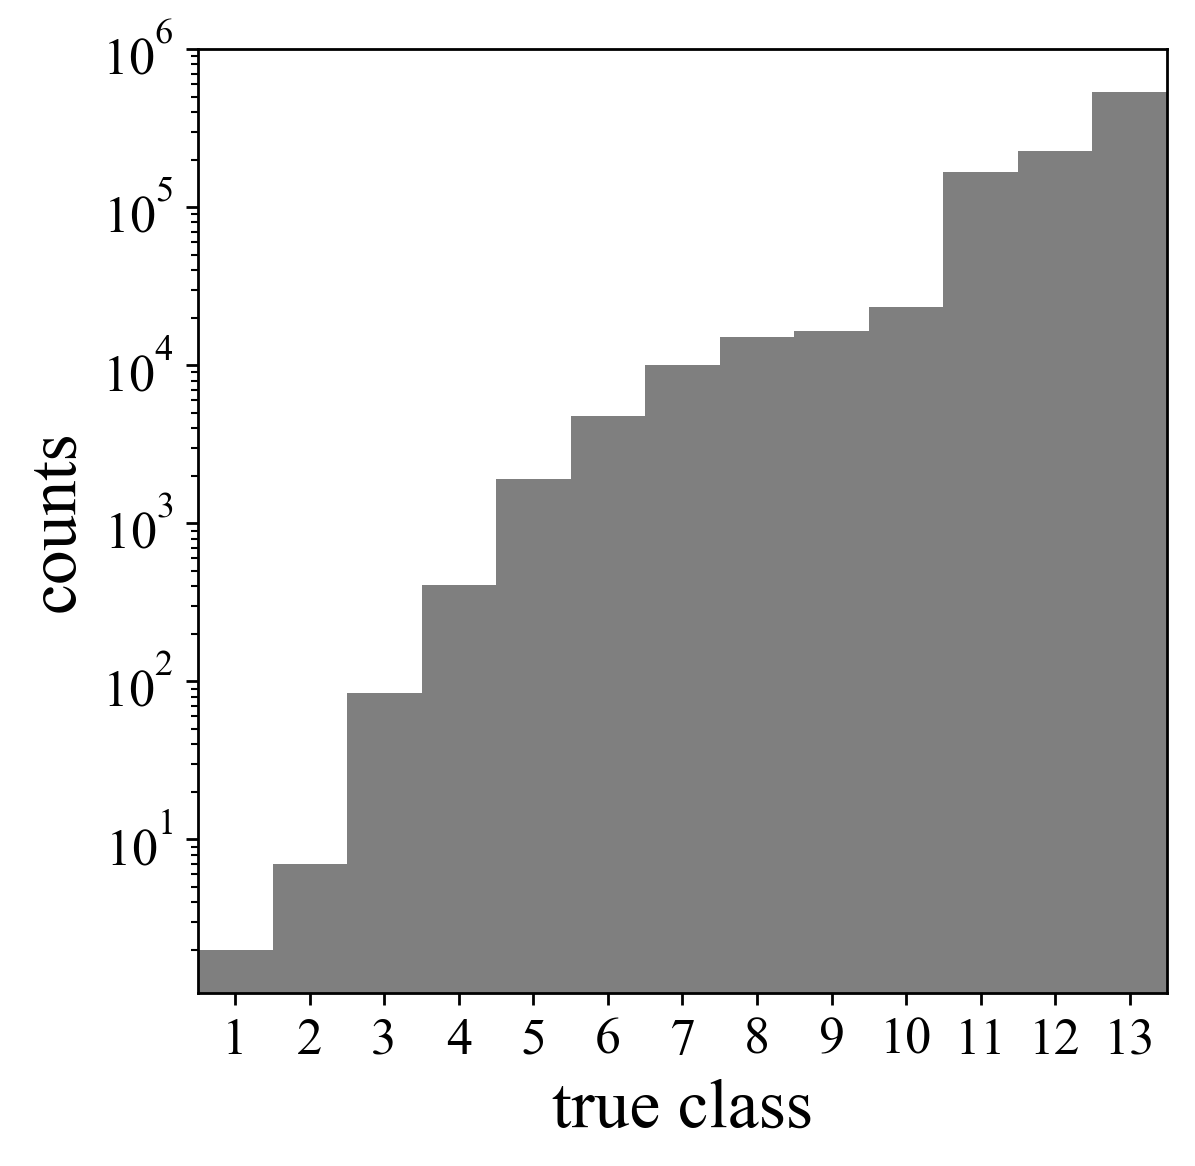
\includegraphics[width=0.45\textwidth]{./fig/complete_counts.png}
		\caption{The numner of objects in a given class as shown as a function of class label, in increasing class size. As expected, the true classes are logarithmically distributed.}
		\label{fig:classdist}
	\end{center}
\end{figure}

Once the true classes have been set, mock classification probabilities for each class are derived using the procedure described in Section~\ref{sec:mockdata}.

\subsection{Mock classification schemes}
\label{sec:mockdata}

In order to test how metrics perform on different classification schemes, we develop `mock classifications', designed to reproduce general responses to a classification challenge.
In particular we will use these mock classifications to investigate how the performance changes when we introduce certain types of failure modes, or \textit{systematics}, to these classificaation schemes.
A robust metric should not reward classification schemes that display these systematic effects.
In other words, we want a metric that is savvy enough to penalize `gaming the system' as much as possible.
%The cases of this section are devised to test if a metric is congruent with our intuitive understanding of what constitutes a good classifier, that it should not reward classifications suffering from the most concerning failure modes, which we will refer to as \textit{systematics} throughout the paper.
%% TODO change systematics to symptoms?
%Our impressions of systematics can be seen as reflections of the conditional probability matrix, a familiar metric of deterministic classification \citep{2012PASP..124.1175B}.
These systematics can be seen as modifications to the confusion matrix, a familiar metric of deterministic classification \citep{bloom_automating_2012}.
The confusion matrix is an $M \times M$ table of observed counts (or, if normalized, frequencies $p(\tilde{m}, m')$) of pairs of estimated class labels $\tilde{m}$ (columns) and true classes $m'$ (rows) computed after a deterministic classification has been performed on some data set with $N$ objects.
Under a binary deterministic classification between positive and negative possibilities, it is natural to count the numbers of true positives $TP$, false positive $FP$ (or Type 1 error), true negative $TN$, and false negative $FN$ (Type 2 error), which can be turned into rates relative to the true numbers of positive and negative instances; these rates may serve as building blocks for more sophisticated metrics of multi-class deterministic classifiers that will be addressed in Section~\ref{sec:methods}.

Though probabilistic classifications are not compatible with the normalized confusion matrix per se, we design tests around proposed normalized confusion matrices exhibiting various symptoms that we anticipate being problematic for \lsst.
Under a deterministic classification scheme, an object with true class $m'$ would have an assigned class $\tilde{m}$ drawn from $p(\tilde{m} \mid m') = p(\tilde{m}, m') / p(m')$, via Bayes' Rule.
We note that the elements of the confusion matrix have values of $N p(\tilde{m}, m')$ and that $N_{m'} / N$ must be known in order to produce a confusion matrix, so we can easily obtain $p(\tilde{m} \mid m')$ to use as the basis for classification probability submissions resulting from a confusion matrix; given its provenance, we refer to the matrix $\mathbb{C}$ comprised of $p(\tilde{m} \mid m')$ as the \textit{conditional probability matrix}.

Since we believe the data contain information about the true class, we can use the appropriate row $\mathbb{C}_{m'}$ of the conditional probability matrix as a proxy for $p(m \mid d)$, without directly classifying lightcurves themselves, which enabled this paper to be written without any knowledge of the \plasticc\ dataset's simulation nor validation.
To emulate the effect of natural variation of information content in different lightcurves, we generate a posterior probability vector $p(m \mid d_{n})$ by taking a Dirichlet-distributed draw
\begin{eqnarray}
  \label{eq:cmtoprob}
  p(m \mid d_{n}) &\sim& \frac{\Gamma(\mathbb{C}_{m_{n}'} \delta)}{\sum_{m'} \Gamma(\mathbb{C}_{m'} \delta)}
\end{eqnarray}
about $\mathbb{C}_{m_{n}'}$, with a small nonnegative perturbation factor $\delta$ and in terms of the gamma function.
% \begin{eqnarray}
%  \label{eq:gamma}
%  \Gamma(\alpha) &=&
% \end{eqnarray}
% \aim{[Rahul: Might be good to have a plot of the pdf when x0 takes values close to 0., something like 0.4, 0.8 and close to 1.0]}

We consider eight `mock classifiers', each of whose effectiveness is described by its conditional probability matrix.
Figure~\ref{fig:mock_cm} shows the conditional probability matrices corresponding to each systematic considered, discussed in detail below.
% TODO: sequential color scheme?
% TODO: letters for panels, refer to them in text
\begin{figure*}
	\begin{center}
    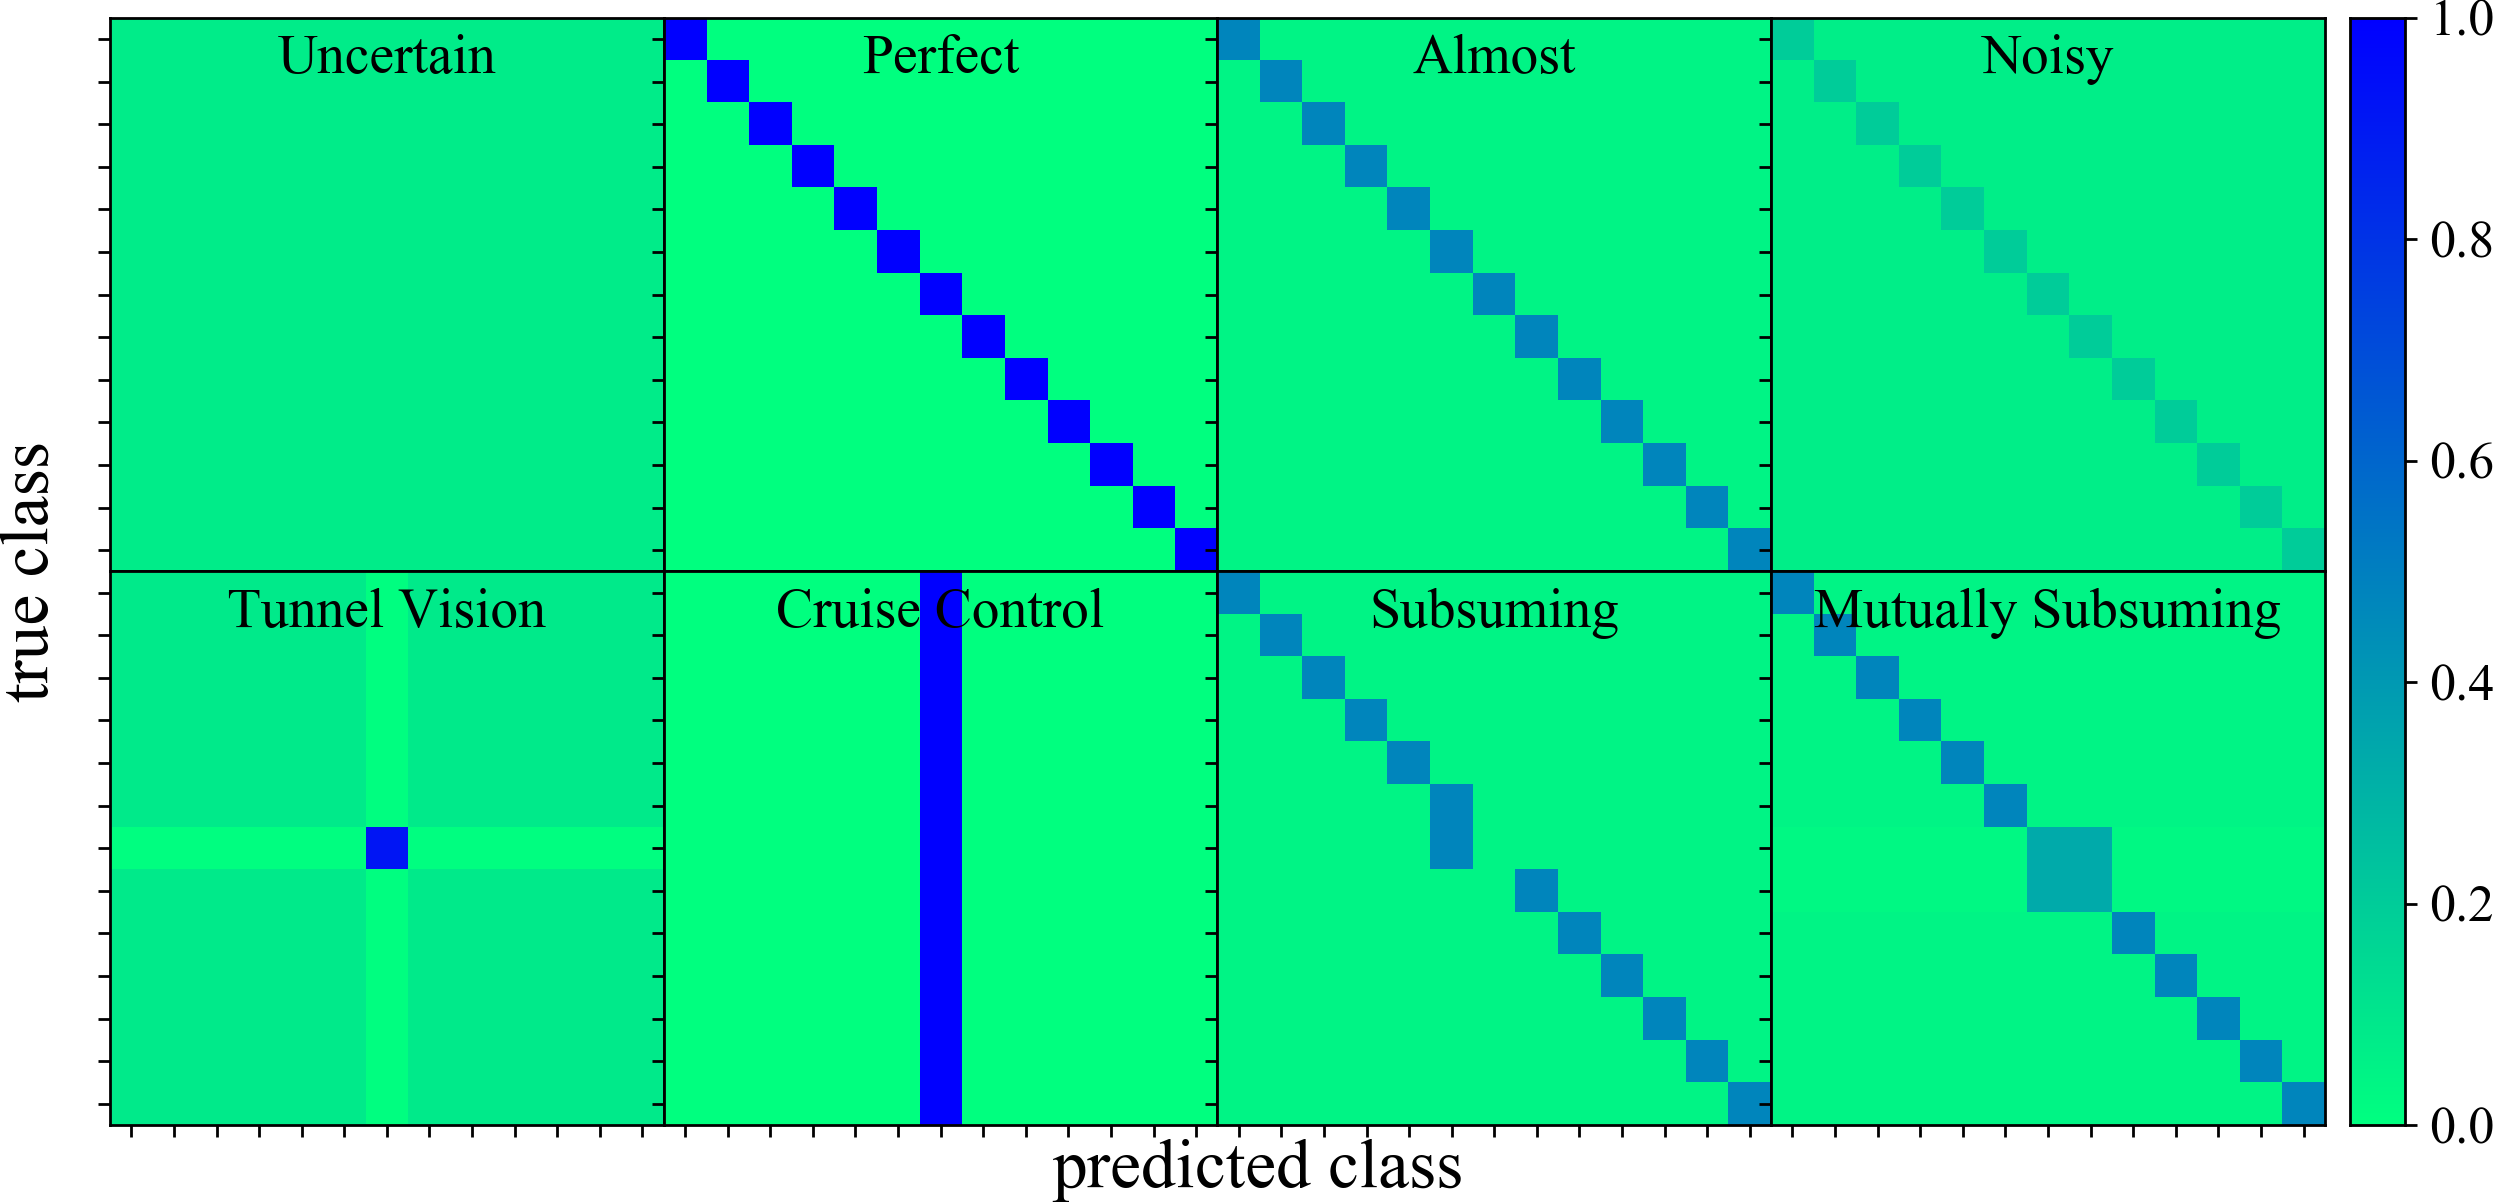
\includegraphics[width=0.8\textwidth]{./fig/all_sim_cm.png}
		\caption{Conditional probability matrices for eight mock classifiers. The left panels show uncertain (top) and perfect (bottom) classifications, while the second panel from the left shows the almost perfect (top) and unbiased but noise (bottom) classifications. The third panel from the left illustrate the perfect classifications that generate Type 1 (False Positive) and Type 2 (False Negative) errors for one class and uniform for all others (the `tunnel classifier', top row), while the bottom row illustrates the classification where all objects are assigned to the same class (the `cruise' classifier). Finally, the panels on the far right show classifications where one class is consistently assigned to another class (subsumed to, top row), and where one consistently assigns another class to one particular class (subsumed from, bottom row). Such classifications arise when one is optimising for a particular science case (e.g., one might prioritize a tunnel classification scheme), or where one object is considered much more `valuable' to classify than others (in which case one would employ a cruise classification scheme.)
%    leftmost top: uncertain classification,
%    leftmost bottom: perfect classifications,
%    left-center top: almost perfect classification,
%    left-center bottom: unbiased classifications,
%    right-center top: 
%    right-center bottom: assigning all objects the same class,
%    rightmost top: consistently assign one class to another,
%    rightmost bottom: consistently assign another class to one class}
		\label{fig:mock_cm}}
	\end{center}
\end{figure*}

For each case, we address:
\begin{enumerate}
  \item What defines the classification error property of this classifier?
  \item Under what conditions is this error property relevant?
  \item What are our expectations of and desires for the way this error property will affect the metric result?
\end{enumerate}

\subsubsection{Uncertain classification}
\label{sec:uncertaindata}

An entirely uniform conditional probability matrix $\mathbb{U}$ (leftmost top panel of Figure~\ref{fig:mock_cm}) would correspond to uniform random guesses for deterministic classification, but, in accordance with Equation~\ref{eq:cmtoprob}, the probability vectors are perturbations away from a uniform distribution across all classes.
The peak values of these probability vectors will correspond to uniform random classifications, however, with $p(m' \mid d)\approx M^{-1}$.
We can consider the \textit{uncertain} classifier as an experimental control for the worst possible classification scheme, bearing in mind that if classifications were somehow anticorrelated with true classes (i.e. consistently misclassifying A as B and B as A), the experimenter could simply reassign the classification labels to improve performance.

\subsubsection{Accurate classification}
\label{sec:accuratedata}

The \textit{perfect} classifier has a diagonal conditional probability matrix $\mathbb{I}$ (leftmost bottom panel of Figure~\ref{fig:mock_cm}), which would correspond to deterministic classifications that are always correct.
In terms of probabilistic classifications, a perfect result would be a probability vector with 1 for the true class and 0 for all other classes.
Due to the random perturbation factor $\vec{e}$, the probability vectors drawn from the perfectly diagonal conditional probability matrix are randomly perturbed away from perfect classifications by the small factor $\delta$, but the class with maximum probability is almost always still the true class, to the tune of $\sim0.96$ with our choice of $\delta$.
This case is also a control, in that \plasticc\ would not be necessary if we believed the perfect classifier were realistically achievable.
In addition to a perfect classifier, we test linear combinations
\begin{eqnarray}
  \label{eq:lincomb}
  \mathbb{C}^{\mathrm{acc}; s} &=& \frac{1}{M+s-1} \left(s\mathbb{I} + \mathbb{U}\right)
\end{eqnarray}
of the perfect and uncertain classifier conditional probability matrices where the contribution of the perfect classifier is greater than that of the uncertain classifier by a factor of $s$.
Deterministic classifications drawn from such a conditional probability matrix would be correct $s$ times as often as they are wrong, and the incorrect guesses would be uncorrelated across classes.
The probability vectors drawn from such conditional probability matrices would have some variability but still mostly have their peak value at the truth.

We consider the case of the \textit{almost perfect} classifier with $s=4$ (left-center top panel of Figure~\ref{fig:mock_cm}) and the \textit{noisy} classifier with $s=2$ (left-center bottom panel of Figure~\ref{fig:mock_cm}), which correspond to $p(m' \mid d)\approx0.82$ and $p(m' \mid d)\approx0.62$ respectively. We expect that the response to variation in $s$ may differ across metrics.
While $s$ would realistically be expected to vary for each class, we do not conduct a systematic investigation of this possibility at this time, and fix $s$ as constant for any given mock classifier.

Indeed, a classifier with different accuracy for each class may be considered a systematic in its own right.
An extreme example of such a classifier could be one with perfect classification performance on one class and uncertain classification on all others; its conditional probability matrix would be uniform except for one row, which would take a value of unity on the diagonal and zero elsewhere.
Such a classifier would have high value to those who study the class with perfect performance and should still be used in the context of \lsst.
For many specific science cases, this type of classifier is desirable, but given the balancing of science cases within \lsst, we take a more measured approach, and require that the \plasticc\ metric must serve the needs of those who study a wide variety of classes for different purposes.
Hence, from the perspective of \plasticc, such a \textit{tunnel vision} classifier (right-center panel of Figure~\ref{fig:mock_cm}) is not something we want to favour with the metric.
%However favoritism is inappropriate for the overall \plasticc\ metric, which must serve the needs of those who study all the classes and for different purposes.

\subsection{Inaccurate classification}
\label{sec:inaccuratedata}

Inaccurate classification in the context of a deterministic classifier is self-explanatory.
If a classifier is systematically inaccurate, its conditional probability matrix has significant probability on off-diagonal elements.
We model inaccurate probabilistic classifications of class $m'$ by using the row of the conditional probability matrix corresponding to class $\tilde{m}$ as the basis for the perturbed probability vector
\begin{eqnarray}
  \label{eq:subsume}
  p(m\ \mid\ m') = p(m\ \mid\ \tilde{m}).
\end{eqnarray}
Class $m'$ is said to be \textit{subsumed} by class $\tilde{m}$ for such a classifier.
The asymmetric relationship between $m'$ and $\tilde{m}$ is illustrated in the rightmost top and bottom panels of Figure~\ref{fig:mock_cm} for class $m'$ being subsumed by class $m'-1$ and class $m'$ subsuming class $m'+1$, respectively.
However, one or more classes could be mutually subsuming if one already has significant off-diagonal probability, as is true for the uncertain classifier.

Subsuming is particularly expected when distinguishing between subtypes of some class, and it is of utmost importance when the subtypes have wholly different science applications.
Classification subtypes that are useful for completely different science cases are found in supernova classification, through e.g., the differences between SN Ia and SN Ibc. SN Ia and SN Ibc are challenging to distinguish, and the former often subsumes the latter in common classifiers, an effect that can be exacerbated by underrepresentation of SN Ibc in available training sets.
However, using SN Ibc in the traditional cosmology analysis done with SN Ia can bias estimates of the cosmological parameters, so the distinction is critical.

Similarly RRc and RRd Lyrae stars have different pulsation modes (RRc stars pulsate in the first overtone, while RRd stars pulsate simultaneously in the fundamental mode and first overtone, and are much more rare than RRc stars), and yet are challenging to separate observationally.
We would like the \plasticc\ metric to identify the strength of a classifier that successfully prevents this kind of error.

An extreme case of inaccurate classification is to classify all objects as the most common class, a particular concern for \plasticc\ given the potential for population imbalance between classes.
For our purposes, it matters not whether the subsuming class is actually the most common or only the most common in the training set.
Such a \textit{cruise control} classifier (right-center bottom panel of Figure~\ref{fig:mock_cm}) counters \plasticc's goal of identifying objects belonging to extremely rare classes, particularly if the metric weights all objects equally.
Though we dampen this systematic by employing per-class weights, described in Section~\ref{sec:weights}, we nonetheless examine its impact under other plausible weighting schemes.

% \subsubsection{Combination of systematics}
% \label{sec:combo}
%
% \begin{figure}
% 	\begin{center}
% 		% 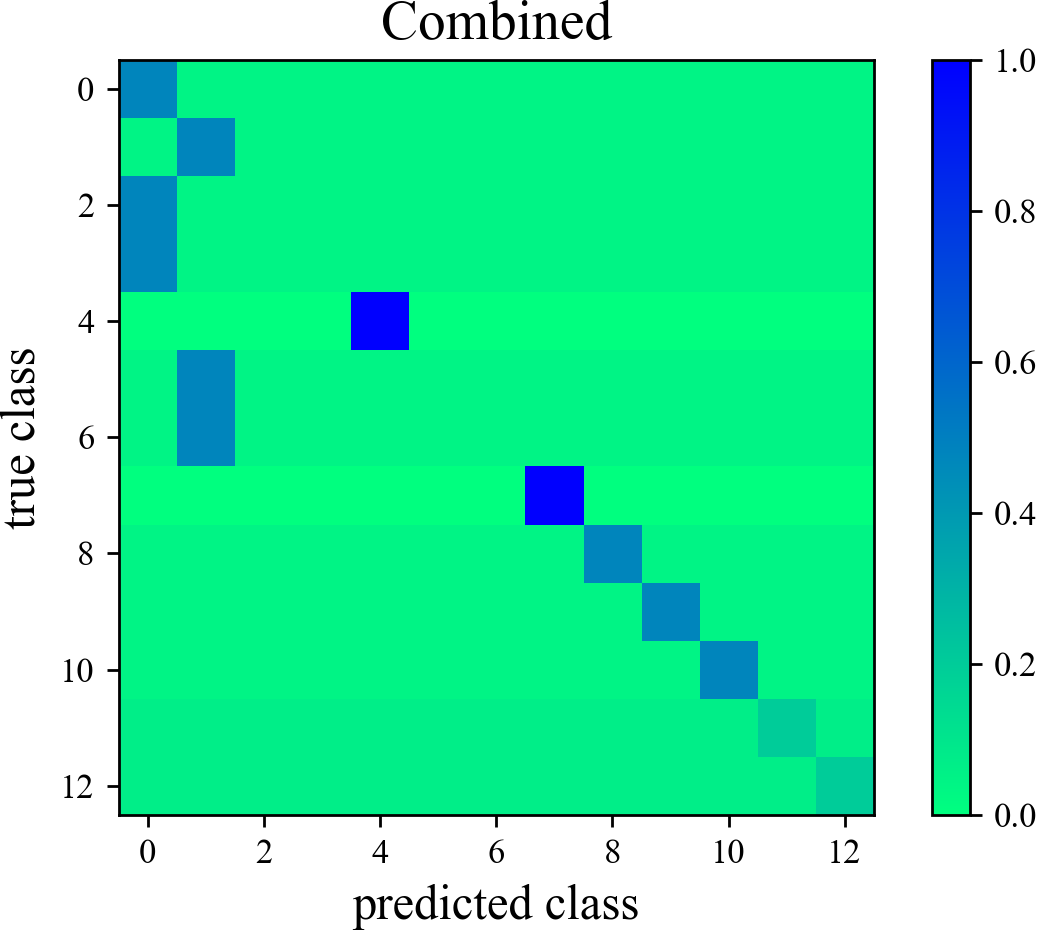
\includegraphics[width=0.45\textwidth]{./fig/Combined.png}
% 		\caption{}
% 		\label{fig:combo_cm}
% 	\end{center}
% \end{figure}

\subsection{Representative classifications}
\label{sec:realdata}

%\aim{This would be more meaningful if we were given the conditional probability matrices of actual submissions to \snphotcc\ and then checked whether the \plasticc\ metric would have designated a different winner.
%Also, it may be more interpretable if we instead use Ashish's conditional probability matrices that have more classes.}
%\aim{This is about representative \textit{training sets} and is irrelevant to this paper.}
% The issue of representative mock classification data is one that concerns classification challenges across a wide range of disciplines.
% The magnitude-limited nature of \lsst\ means that our test data will always be non-representative.
% Hence the \plasticc\ data will follow the real world as closely as possible.

In order to understand the performance of classifiers on simulated data sets approximating reality, we calculate the values of our metric candidates on realistic classification of a precursor supernova classification challenge.
The Supernova Photometric Classification Challenge (\snphotcc) \citep{kessler_supernova_2010} focused on classifying the lightcurves of a heterogenous population into a limited number of subclasses, with a goal of identifying one particular type of object for a single scientific application.
\snphotcc\ provided a data set of three types, SN Ia, SN II, and SN Ibc.
The original metric was based solely on correctly classifying SN Ia deterministically, with no penalty for confusing SN II for SN Ibc and vice versa, nor was there any notion of a confidence in a classification.
The \snphotcc\ attracted diverse classification approaches, including $\chi^{2}$ fits of the supernova lightcurves to publicly available templates \citep{nugent_kcorrections_2002}, physical models \citep{conley_sifto:_2008}, and empirical models, as well as alternatives to curve-fitting such as outlier identification on the training set Hubble diagram, dimensionality reduction, and clustering.
% TODO cite InCA?
% A general light curve shape (rather than one motivated by the physical differences between SNeIa and core collapse SNe) was assumed by some competitors and then a kernel density estimation was performed over the fit parameters, with various approaches employed including boosting over the feature space.
Machine learning was also employed, using features such as the light-curve slopes to produce a predictive model for the training data.
In short, \snphotcc\ attracted physically motivated template-based methods sensitive to the differences between the test data and the template set as well as those based on decomposition of the light curves into generic features at risk of neglecting available physical information.
% TODO need citations of ML submissions to SNPhotCC
%, which are prone to bias given non-representativity of the test data and agnostic
After the \snphotcc\ concluded, the lightcurves became a testbed for a suite of machine learning classifiers.
We consider one such compilation of methods, as presented in \citet{lochner_photometric_2016}, whose conditional probability matrices are shown in Figure~\ref{fig:snphotcc_cm}.
% TODO what are the 3 classes?
These classification algorithms include a wavelet decomposition of the lightcurves to construct the features over which to classify (\citet{newling_statistical_2011}, bottom row) and template-based classification procedures (\citet{sako_photometric_2011}, top row), each paired with Boosted Random Forest (BF), K-Nearest Neighbors (KNN), Naive Bayes (NB), Support Vector Machine (SVM), and Neural Network (NN) machine learning algorithms (columns).
While the complexity of entries to the \snphotcc\ was greater than this subset, we use these illustrative examples as a useful comparison set over which to assess the performance of the approaches under our metric scheme.

\begin{figure*}
	\begin{center}
    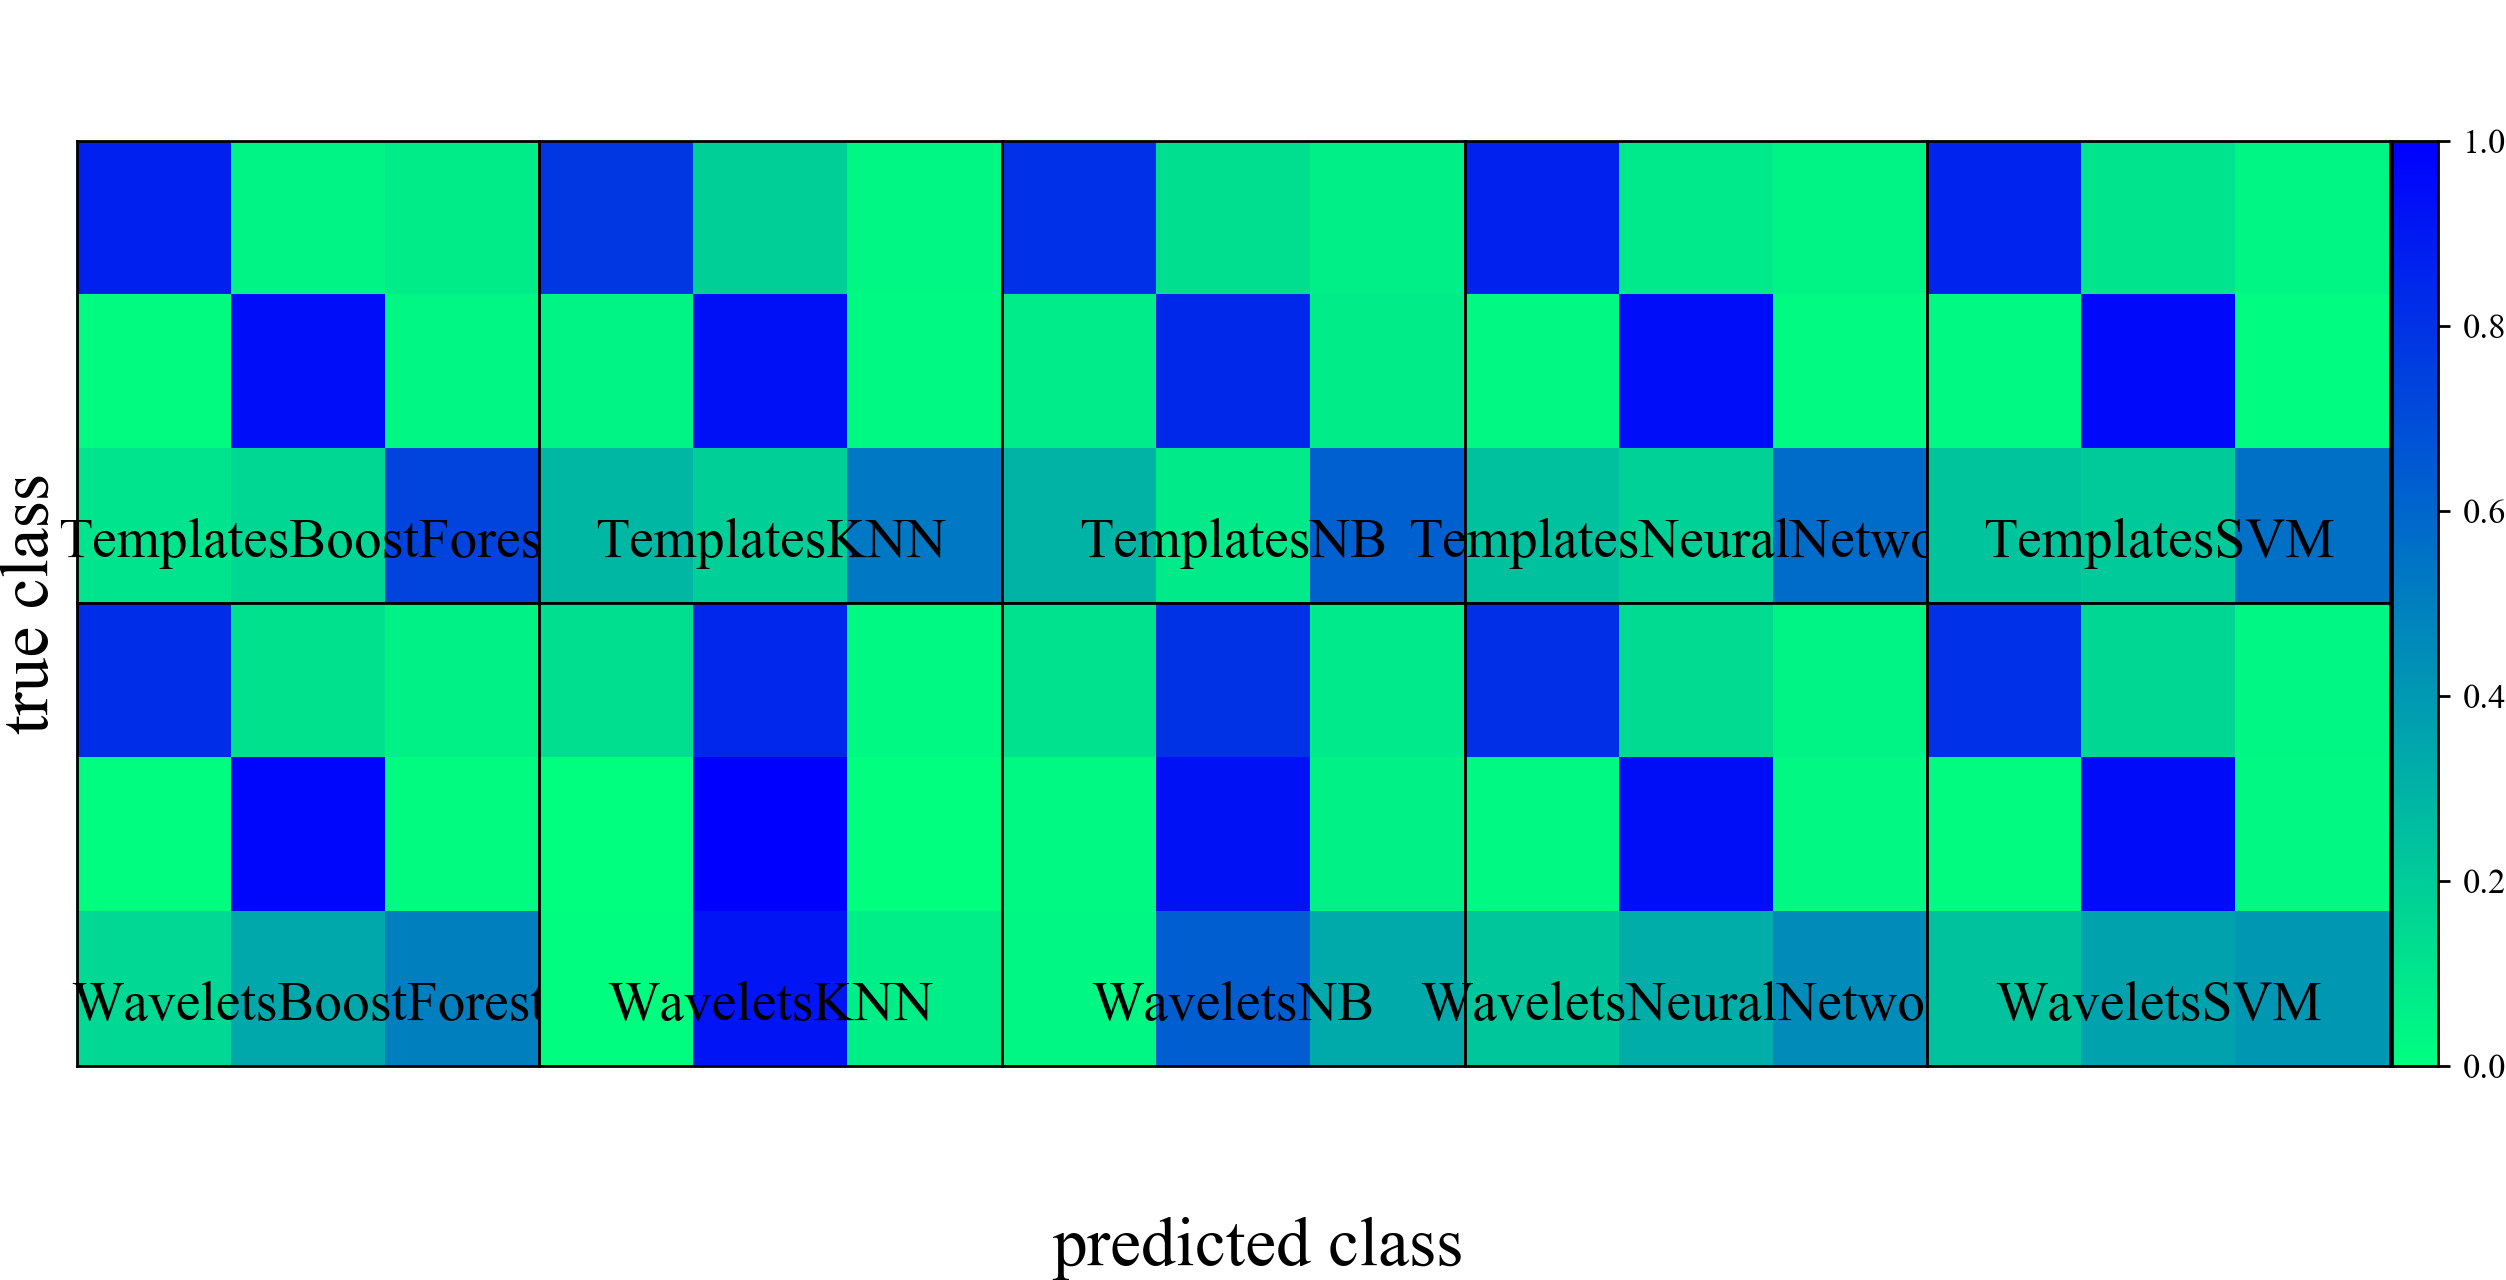
\includegraphics[width=\textwidth]{./fig/all_snphotcc_cm.png}
		\caption{Conditional probability matrices of the \citet{lochner_photometric_2016} methods applied to the \snphotcc\ dataset.
    Top row: five machine learning methods applied to template decompositions.
    Bottom row: the same five machine learning methods applied to wavelet features.}
		\label{fig:snphotcc_cm}
	\end{center}
\end{figure*}

We draw attention to the presence of the systematics introduced in Section~\ref{sec:mockdata} in these realistic classification results.
Note that the ``WaveletsNN'' and ``WaveletsNB'' methods both suffer from the cruise control systematic.
Nearly all the others exhibit classifications that are almost perfect for the first class, perfect for the second class, and noisy for the third.
\aim{What are these classes?}

% \subsubsection{Unknown dataset}
% \label{sec:mystery}
%
% \begin{figure*}
% 	\begin{center}
% 		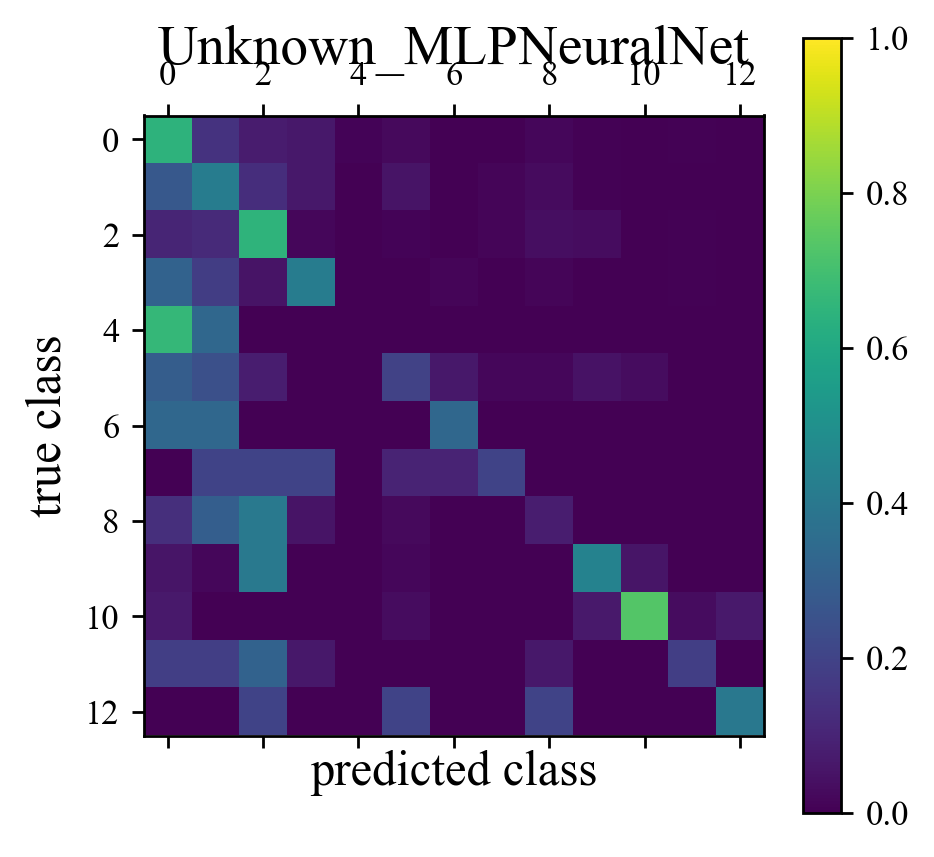
\includegraphics[width=0.3\textwidth]{./fig/Unknown_MLPNeuralNet_cm.png}
% 		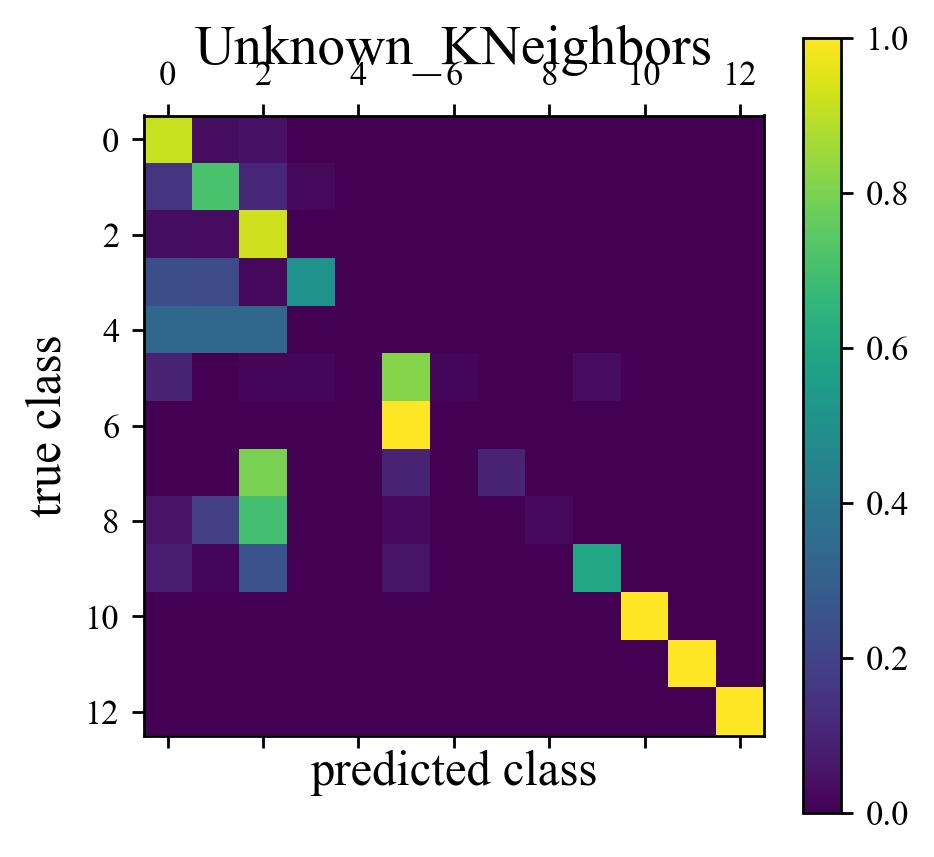
\includegraphics[width=0.3\textwidth]{./fig/Unknown_KNeighbors_cm.png}
% 		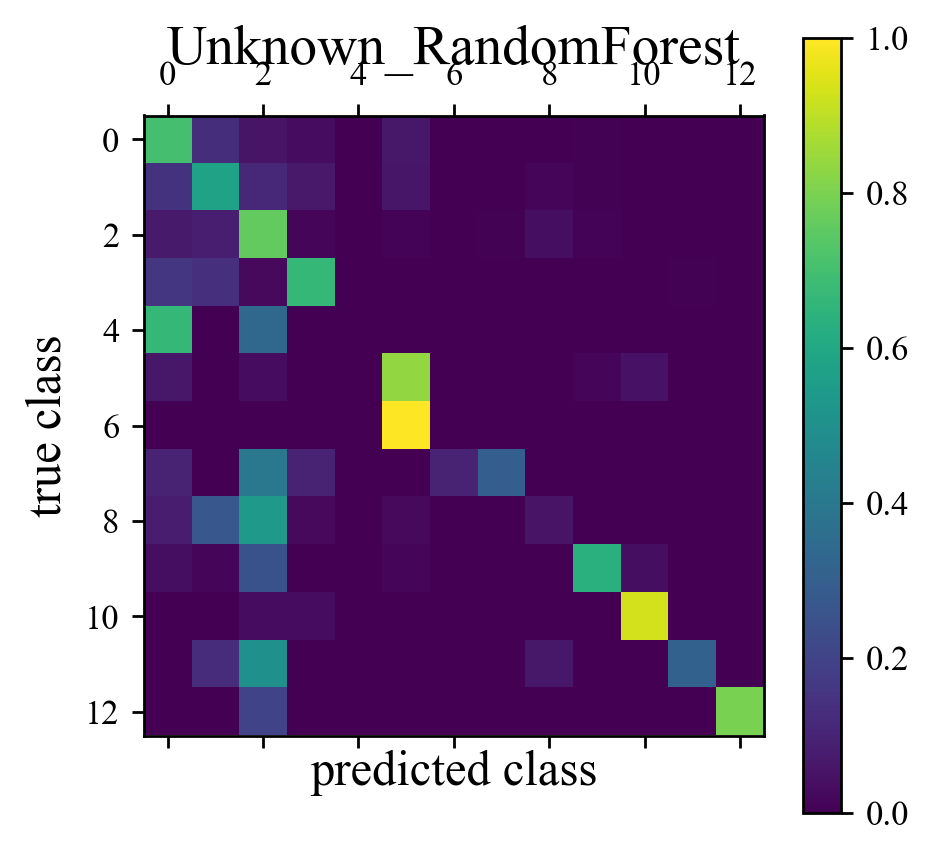
\includegraphics[width=0.3\textwidth]{./fig/Unknown_RandomForest_cm.png}
% 		\caption{}
% 		\label{fig:unknown_cm}
% 	\end{center}
% \end{figure*}
